\FloatBarrier
\chapter{Uitwendige stroming}
\label{sec:Uitwendige stroming}

	\FloatBarrier
	\section{Inleiding}
	\label{sec:Uitwendige stroming Inleiding}
In dit hoofdstuk zullen een aantal hulpiddelen voor het beschijven van stroming uitwendig aan een voorwerp beschreven worden. Als eerste wordt een analytische methode voor niet viskeuze tweedimensionale stroming besproken. Nadien wordt het gedrag van een viskeuze uitwendige stroming beschreven. In het laatste deel wordt de stroming rond een vleugelprofiel, een in de ingenieurstoepassing vaak voorkomende vorm, beschreven.

	\FloatBarrier
	\section{Potentiaalstroming}
	\label{sec:Potentiaalstroming}

Uit de vectorveld analyse weten we dat wanneer een vectorveld rotatievrij is er een scalaire potentiaalfunctie bestaat waaruit de componenten van het vectorveld kunnen worden afgeleid.
\npar
Wanneer er geen viskeuze krachten op een flu\"idum inwerken zal de rotatie van het snelheidsveld $0$ zijn. Het met andere woorden: het snelheidsveld is rotatievrij. Er zal dus een potentiaalfunctie bestaan waaruit de componenten van het snelheidsveld kunnen worden afgeleid.
\npar
Dit vereenvoudigt de oplossing van het snelheidsveld voor gegeven randvoorwaarden aanzienlijk. Voor een tweedimensionale niet-samendrukbare stroming moet normaalgezien een stelsel van 2 gekoppelde parti\"ele differentiaalverlijkingen opgelost worden (\'e\'en voor elke richting). Onder de voorwaarden van potentiaalstroming vereenvoudigt dit to \'e\'en parti\"ele differentiaalverlijking.
		\subsection{Stroomfunctie}
Beschouw een willekeurige tweedimensionale stroming met stroomlijnen zoals in Figuur \ref{fig:Stroomfunctie}.
\begin{figure}[htb]
	\centering
	%\includesvg{fig/uitwendige_stroming/Stroomfunctie}
	\caption{Stroomlijnen van een tweedimensionale stroming}
	\label{fig:Stroomfunctie}
\end{figure}
Berekenen we nu het debiet $\diff \dot{V}$ tussen twee stroomlijnen op een afstand $\diff n$.
\begin{equation}
	\diff \dot{V} = v \diff n
\end{equation}
De snelheid kan beschreven worden door zijn 2 componenten, $v_x$ en $v_y$. We kunnen de vector $\diff n$ beschrijven met zijn componenten $dx$ en $dy$ (Figuur \ref{fig:Stroomlijn coordinaten}). De componenten van $\vt{v}$ loodrecht op het oppervlak $\diff n$ kunnen nu berekend worden als:
\begin{eqnarray}
	v_{x,\perp} &=&  v_x \frac{\diff y}{\diff n} \\
	v_{y,\perp} &=& -v_y \frac{\diff x}{\diff n}
\end{eqnarray}
Hierin wordt bij $\diff x$ een min teken toegevoegd aangezien $\diff x$ zoals hier getekend een negatieve waarde zal hebben. Het debiet wordt nu:
\begin{equation}
	\diff \dot{V} = v_x \frac{\diff y}{\diff n} \diff n - v_y \frac{\diff d}{\diff n} = v_x \diff y - v_y \diff x
	\label{eqn:debiet tussen stroomlijnen}
\end{equation}
Beschouw nu de onbekende stroomfunctie $\psi$ die een scalaire functie is in $x$ en $y$. De verandering van deze stroomfunctie kan met behulp van de kettingregel gescheven worden in functie van zijn parti\"ele afgeleiden naar de twee co\"ordinaten:
\begin{equation}
	\diff \psi = \frac{\partial \psi}{\partial x} \diff x + \frac{\partial \psi}{\partial y} \diff y
	\label{eqn:verandering van de stroomfunctie}
\end{equation}
Indien we nu (\ref{eqn:debiet tussen stroomlijnen}) en (\ref{eqn:verandering van de stroomfunctie}) vergelijken zien we dat we de stroomfunctie kunnen defini\"eren als het debiet tussen een stroomlijn en een vaste referentie stroomlijn. De snelheids componenten kunnen dan uit de stroomfunctie afgeleid worden als:
\begin{eqnarray}
	v_x &=&  \frac{\partial \psi}{\partial y} \\
	v_y &=& -\frac{\partial \psi}{\partial x}
\end{eqnarray}
\begin{figure}[htb]
	\centering
	\includesvg{fig/uitwendige_stroming/Stroomlijnen}
	\caption{Vectoren van de stroomlijn co\"ordinaten}
	\label{fig:Stroomlijn coordinaten}
\end{figure}
Een belangrijke eigenschap van de stroomfunctie is dat contouren van constante stroomfunctie de stroomlijnen beschrijven. Dit kan rechtstreeks afgeleid worden uit de interpretatie van de stroomfunctie als debiet.
\npar
Uit de vector analyse volgt dat voor een rotatievrije stroming de stroomfunctie moet voldoen aan de Laplacevergelijking.
\begin{equation}
	\frac{\partial^2 \psi}{\partial x^2} + \frac{\partial^2 \psi}{\partial y^2} = 0
	\label{eqn:laplacevergelijking}
\end{equation}
Analytische oplossingen voor deze vergelijking bestaan voor een groot aantal verschillende randvoorwaarden. Een bijkomend voordeel van deze formulering is dat de Laplacevergelijking een lineaire parti\"ele differentiaalvergelijking is. Hierop is het superpositieprincipe van toepassing. Een lineaire combinatie van oplossingen zal dus ook voldoen aan de vergelijking. Met behulp hiervan kunnen een aantal verschillende problemen analytisch behandeld worden.
	\FloatBarrier
	\section{Grenslagen}
	\label{sec:Grenslagen}
Beschouw vlakke plaat waar langs \'e\'en zijde een viskeus flu\"idum over stroomt (Figuur \ref{fig:Laminaire grenslaag}). Vlak voor de plaat is de stroming uniform, de snelheid varieert niet met de hoogte. Bij het begin van de plaat zullen de deeltjes het dichtst bij de plaat door de wrijvingskrachten afgeremd worden tot stilstand. De deeltjes verder van de plaat worden op deze plaats echter nog niet beinvloed door de plaat. Wanneer het flu\"idum verder over de plaat stoomt zullen de deeltjes die iers verder van de plaat stromen ook afgeremd worden door de deeltjes het dischtst bij de plaat. De deeltjes ver van de plaat ondervinden echter nog steeds geen invloed van de plaat.
\begin{figure}[htb]
	\centering
	\includesvg{fig/uitwendige_stroming/Laminaire_grenslaag}
	\caption{Vorming van een grenslaag bij stroming over een vlakke plaat}
	\label{fig:Laminaire grenslaag}
\end{figure}
\npar
Hoe verder we van het begin van de plaat kijken hoe groter de zone waarin de fui\"idum deeltjes het effect van de plaat ondervinden zal worden. De zone waarin de snelheid van het fui\"idum kleiner is dan 99\% van de ongestoorde snelheid wordt de \emph{grenslaag} genoemd.
\npar
Bij elke viskeuze stroming die in aanraking komt met een wand op een andere snelheid wordt een grenslaag gevormd. Deze vormt een handig hulpmiddel voor de analyse van viskeuze stromingen rond voorwerpen aangezien slechts een gedeelte van het stroomveld in rekening gebracht moet worden (het gedeelte binnen de grenslaag). De bepaling van de dikte van een grenslaag is echter niet zo eenvoudig en zal niet behandeld worden in deze cursus.
\npar
Wanneer de dikte van de grenslaag echter gekend is kan gemakkelijk een snelheidsprofiel verondersteld worden. Hieruit kunnen dan de schuifspanningen aan de wand berekend worden en uit deze volgt de viskeuze weerstandskracht die de vloeistof op de wand uitoefent.
\npar
In het voorgaande voorbeeld liepen alle snelheidsvectoren in dezelfde richting. Indien we de stroomlijnen in deze stroming zouden tekenen is te zien dat deze allemaal parallel lopen. De stroming wordt als het ware door de ongestoorde snelheid gedwongen in verschillende lagen te stromen. Zo'n stroming noemen we \emph{laminair}. Wanneer ons nog verder over de wand verplaatsen zal de grenslaag steeds dikker worden. Op een gegeven moment wordt de grenslaag zo dik dat de stroming binnen de grenslaag onstabiel wordt. Er zullen variaties van de grootte en richting snelheid optreden naargelang de plaats en het tijdstip waarop we kijken (Figuur \ref{fig:Turbulente grenslaag}). We noemen dit een turbulente grenslaag.
\begin{figure}[htb]
	\centering
	\includesvg{fig/uitwendige_stroming/Turbulente_grenslaag}
	\caption{Vorming van een turbulente grenslaag bij stroming over een vlakke plaat}
	\label{fig:Turbulente grenslaag}
\end{figure}
\npar
In een turbulente grenslaag zal het flu\"idum niet meer netjes in lagen stromen. Zeer dicht bij de band zal er wel een kleine zone van laminaire stroming zijn. Hier zorgt de wand voor de stabilisatie van de stroming. We noemen deze laag de laminiare sublaag.
\npar
In een turbulente grenslaag wordt de weerstandskracht niet enkel meer bepaald door de viscositeit. Buiten de laminaire sublaag beweegt de vloeistof onregelmatig door elkaar. Er zal dus convectieve impulsoverdracht plaatvinden over de lagen heen. De schuifspanning wordt hier veroorzaakt door de onregelmatigheid van de snelheden en wordt de turbulente schuifspanning of Reynoldsspanning genoemd. Het correct bepalen van deze spanningen is tot op heden niet mogelijk en vormt \'e\'en van de blijvende uitdagingen in de flu\"idummechanica. Er bestaan wel meerdere ad hoc benaderingen voor de Reynoldsspanningen die in bepaalde gevallen voldoende betrouwbare resultaten geven.
\npar
Binnen de laminaire sublaag zal de laminaire schuifspanning terug domineren. Aangezien er in het turbulente gedeelte meer impuls overdracht is zal een turbulent snelheidsprofiel steeds een grotere gradi\"ent hebben in de buurt van de wand en vlakker zijn verder van de wand. De uitgeoefende viskeuze weerstandskracht is dan ook steeds groter bij een turbulente stroming dan bij een laminaire stroming.
		
		\subsection{Turbulentie}
Wanneer het Reynoldsgetal in een stroming groot genoeg is zal de stroming turbulent worden. Het snelheidsveld dat de stroming beschrijft bevat dan schijnbaar willekeurige variaties in grootte en richting van de snelheid. Het fenomeen werd als eerste beschreven en gequantificeerd door Osbourne Reynolds voor een stroming in een buis. In een turbulente stroming ontstaan onstabiele wervels van verschillende grootteordes die zorgen voor de fluctuaties in de snelheid. Een turbulente stroming wordt nog steeds beschreven door de Navier-Stokes vergelijking (\ref{eqn:navier-stokes vergelijkingen}). Door de niet lineaire convectieve termen in de deeltjesversnelling ($v_i \frac{\partial v_j}{\partial x_i}$) is het bekomen van een oplossing voor de vergelijkingen tot nog toe niet mogelijk. Wel bestaan er technieken die het numeriek benaderen van turbulente stroming modelijk maken.

De oorsprong van de wervels kunnen we illustreren met een eenvoudig voorbeeld. Beschouw een stroming met een sinusvormige verstoring in de $x$-richting ($v_x = \sin(\omega x)$). De convectieve term van de deeltjesversnelling in de $x$-richting wordt nu:
\begin{equation}
	v \frac{\partial v}{\partial x} = \omega \sin(\omega x) \cos(\omega x) = \frac{1}{2} \omega \sin( 2 \omega) 
\end{equation}
Een aanwezige verstoring wordt dus met een half zo kleine golflengte overgedragen naar de versnelling. Er wordt met andere woorden energie overgedragen naar kleinere golflengten en hogere frequenties. Hierdoor zal een globale verstoring evolueren tot een variatie in snelheid op zeer kleine schaal. Wanneer de stroming viskeus is zullen vanaf een bepaalde (kleine) schaal de ossilaties gedempt worden door de viskeuze krachten. Het Reynolds getal (verhouding tussen traagheidskrachten en viskeuze krachten) zal dus een goede maatstaf zijn voor het inschatten van turbulentie. De Reynoldsgetallen waarbij turbulentie optreed zijn echter sterk afhankelijk van de specifieke situatie. Bij de grenslaagstroming over een vlakke plaat zoals hierboven beschreven zal turbulentie optreden vanaf een Reynoldsgetal van 350000 - 1000000 \cite{Schlichting1979}. Het Reynoldsgetal word in dit geval gedefinieerd als:
\begin{equation}
	Re_x = \frac{v x}{\nu}
\end{equation}
Hierin is $x$ de afstand van het beschouwde punt tot de rand van de plaat. Een voorbeeld van snelheidsvectoren van een turbulente stroming over een vlakke plaat is gegeven in Figuur \ref{fig:Turbulente grenslaag voorbeeld}.
\begin{figure}[htb]
	\centering
	\includesvg[15cm]{fig/uitwendige_stroming/Turbulente_grenslaag_voorbeeld}
	\caption{Snelheidsvectoren opgemeten bij een turbulente grenslaag over een vlakke plaat \cite{Tomkins1997}.}
	\label{fig:Turbulente grenslaag voorbeeld}
\end{figure}

	\FloatBarrier
	\section{Loshechting}
	\label{sec:Loshechting}
	
Beschouw de stroming rond een cilinder. Wanneer we de stroomlijnen tekenen voor verschillende Reynolds getallen kunnen we enkel duidelijke regimes onderscheiden (Figuur \ref{fig:Sroomlijnen bij stroming rond een cilinder}).
\npar
Bij zeer lage snelheden zullen de viskeuze krachten overheersen (Figuur \ref{fig:cilinder Re 1} en Figuur \ref{fig:cilinder Re 10}). De stroming is zeer viskeus en de snelheid zal in het gehele stroomveld het effect van de cilinder ondervinden. De grenslaag is in dit geval zeer groot.
We kunnen een wrijvingsco\"effici\"ent berekenen als:
\begin{equation}
	C_d = \frac{F_d}{1/2 \rho v^2 A_{\perp}}
	\label{eqn:wrijvingscoefficient}
\end{equation}
Deze zal bij lage Reynolds getallen zeer groot zijn en sterk afhankelijk zijn van het Reynoldsgetal (Figuur \ref{fig:cilinderstroming_cd}). De wrijving wordt echter slechts gedeeltelijk door viskeuze wijving (ten gevolge van de grenslaag) veroorzaakt. Het overige gedeelte wordt veroorzaakt door het drukverschil tussen de voor en achterzijde.
\begin{figure}[htb]
	\centering
	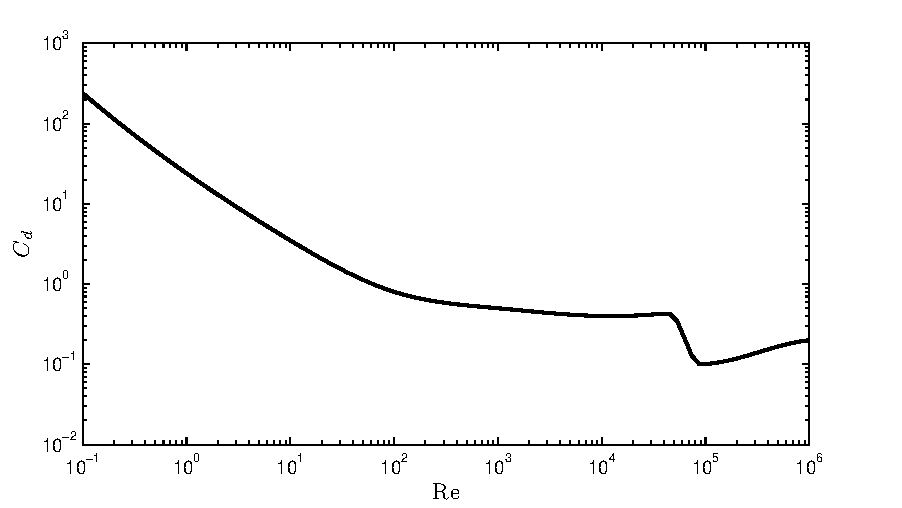
\includegraphics{cilinderstroming_Cd.pdf}
	\caption{Wrijvingsfactor bij stroming van rond een cilinder }
	\label{fig:cilinderstroming_cd}
\end{figure}
\begin{figure}[htb]
	\centering
	\includesvg{fig/uitwendige_stroming/loshechting}
	\caption{Afscheiding van een viskeuze stroming onder invloed van een positieve drukgradi\"ent}
	\label{fig:afscheiding}
\end{figure}
\begin{figure}[htb]
	\centering
	\subfigure[Re = 1]{
		\label{fig:cilinder Re 1}
		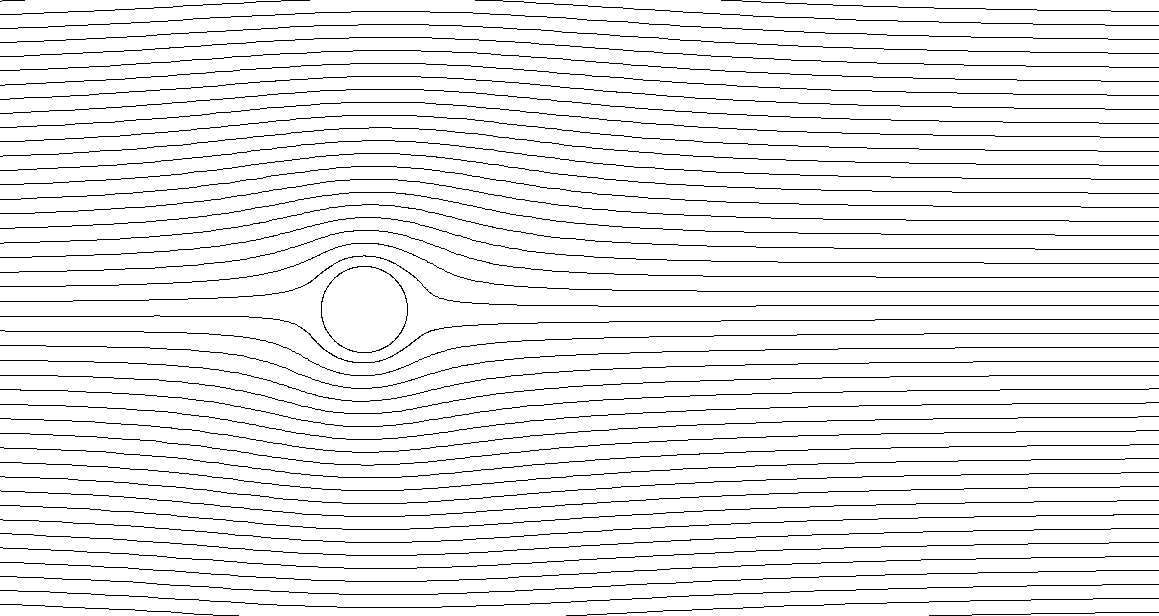
\includegraphics[height=0.2\textwidth]{Stroomfunctie_Re1_bw.png}
	} \quad
	\subfigure[Re = 10]{
		\label{fig:cilinder Re 10}
		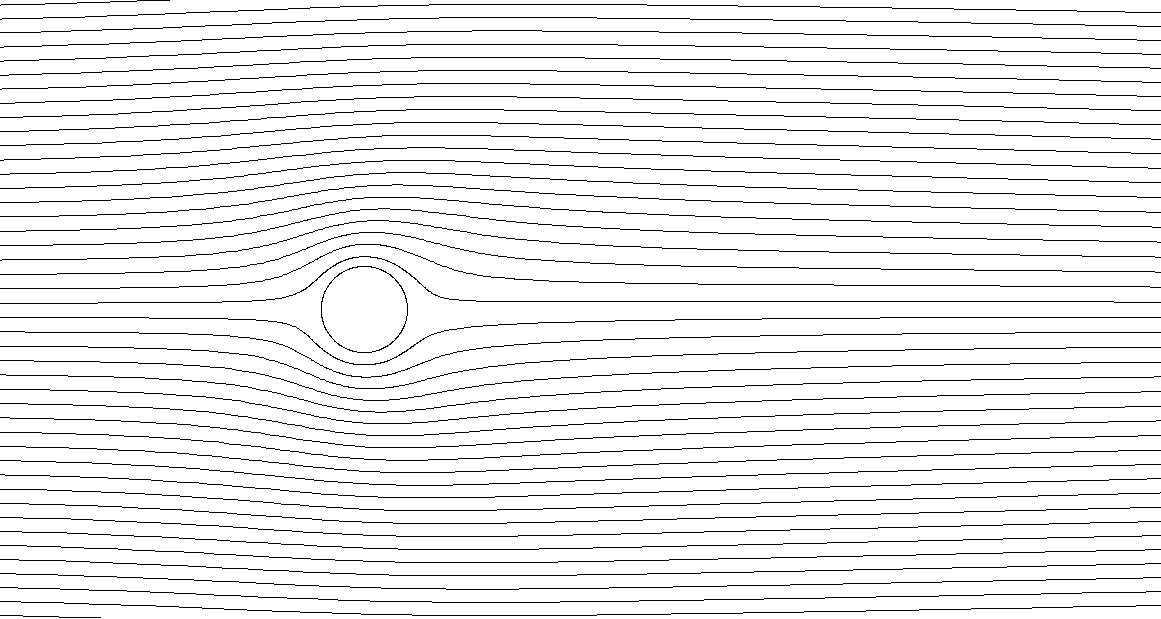
\includegraphics[height=0.2\textwidth]{Stroomfunctie_Re10_bw.png}
	}
	\\
	\subfigure[Re = 100]{
		\label{fig:cilinder Re 100}
		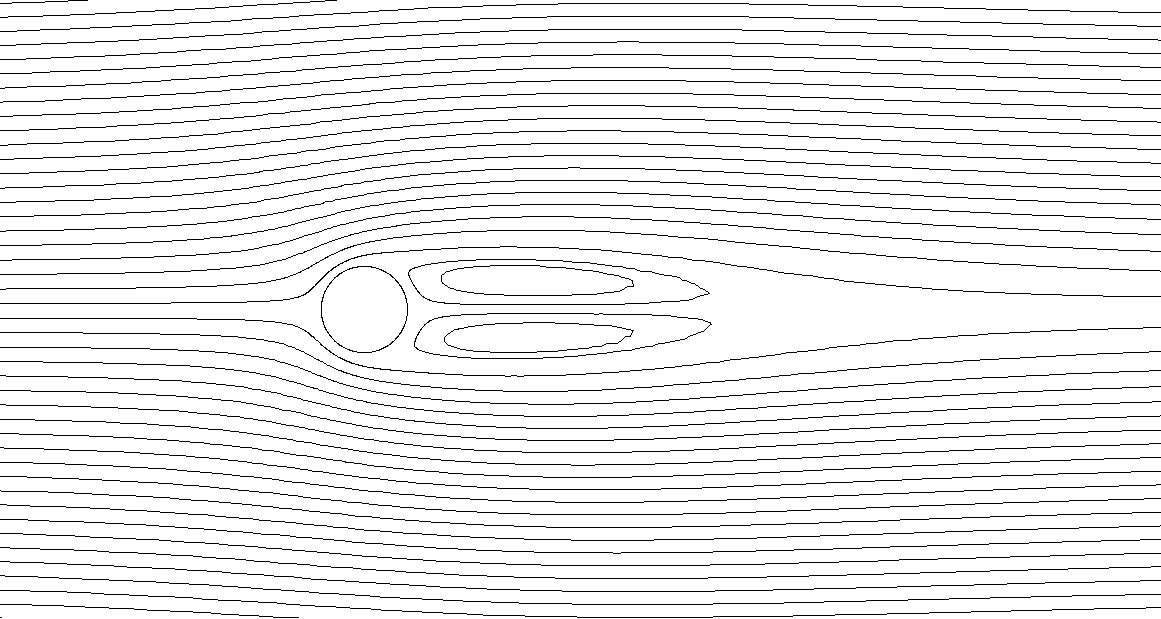
\includegraphics[height=0.2\textwidth]{Stroomfunctie_Re100_bw.png} 
	} \quad
	\subfigure[Re = 1000]{
		\label{fig:cilinder Re 1000}
		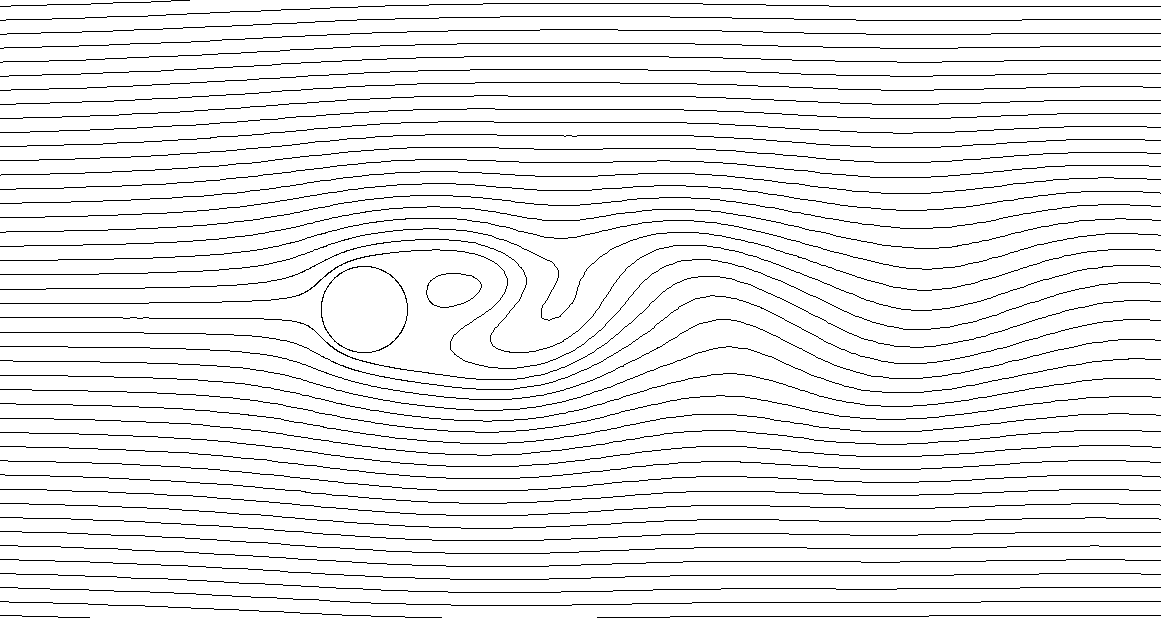
\includegraphics[height=0.2\textwidth]{Stroomfunctie_Re1000_bw.png}
	}
	\\
	\subfigure[Re = 100000]{
		\label{fig:cilinder Re 100000}
		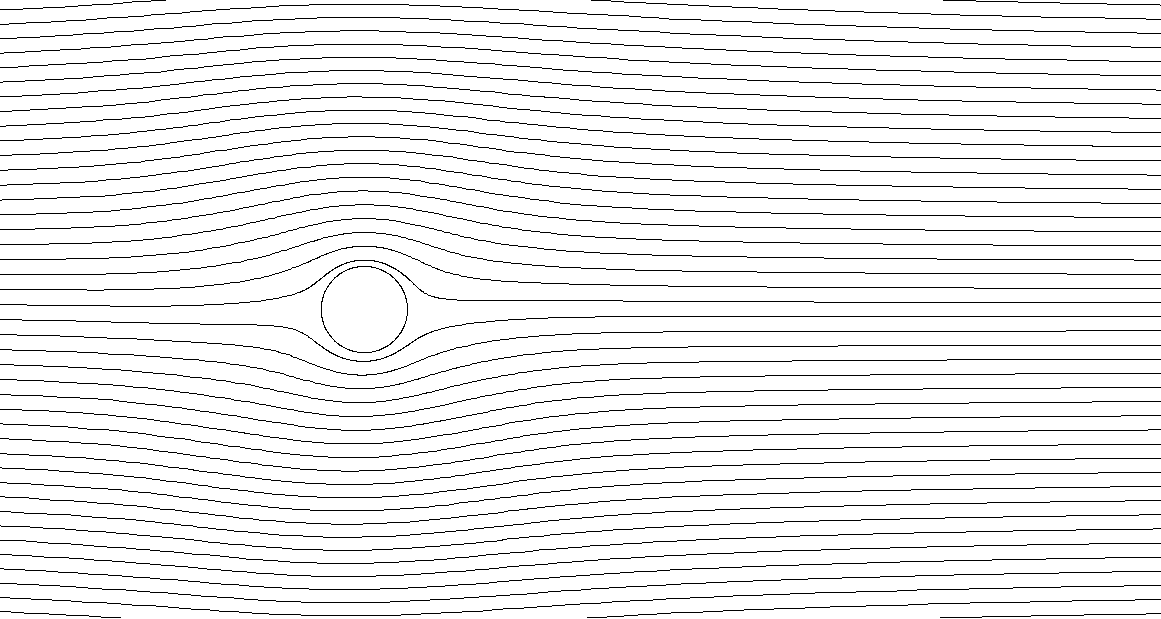
\includegraphics[height=0.2\textwidth]{Stroomfunctie_Re10000_bw.png}
	}
	\caption{Stroomlijnen bij stroming rond een cilinder voor verschillende Reynolds getallen}
	\label{fig:Sroomlijnen bij stroming rond een cilinder}
\end{figure}
\npar
Bij hogere Reynolds getallen zien we dat er een zog met circulatie stroming achter de cilinder ontstaat (Figuur \ref{fig:cilinder Re 100}). De wrijvingsco\"effici\"ent daalt ook niet meer zo sterk als verwacht onder invloed van de dalende viskeuze krachten. Dit verschijnsel wordt \emph{afscheiding} of \emph{loshechting} genoemd. Bij gemiddeld grote Reynolds getallen zal het gedeelte waarin afscheiding optreedt stabiel zijn. Bij hogere Reynolds getallen zal de stroming beurtelings langs de ene en de andere zijde loshechten waardoor er wervelingen ontstaan die zich in de stroming voortplanten (Figuur \ref{fig:cilinder Re 1000}). Deze periodische loshechting brengt een periodische kracht loodrecht op de gemiddelde stroomrichting met zich mee. De frequentie van het loshechten kan gekarakteriseerdworden door het Strouhal getal ($\text{St} = fD/v$) dat voor de stroming rond een cilinder ongeveer 0.2 is.
\npar
Bij nog hogere waarden van het Reynolds getal zal de afgescheide zone achter de cilinder terug verkleinen terwijl ook de wrijvingsco\"effici\"ent terug daalt (Figuur \ref{fig:cilinder Re 100000}).
\npar
Om deze waarnemingen te verklaren bekijken we ook de stroming bij de afwezigheid van viskeuze krachten (potentiaalstroming). In deze situatie ontstaat er een hoge druk zone voor de cilinder met een stagnatiepunt waar de stroming helemaal tot stilstand komt. Aan de zijkanten (op 90\degree en 270\degree) zal de snelheid van het flu\"idum het grootst zijn. De druk is hier minimaal. wanneer we verderop in de stroming kijken zal aan de achterzijde van de cilinder (180\degree) ook een stagnatiepunt zijn waar de snelheid $0$ is en de druk maximaal. Er wordt met andere woorden energie omgezet van druk aan de voorzijde van de cilinder naar kinetische energie aan de randen en terug naar druk aan de achterzijde van de cilinder. Aan de achterzijde van de cilinder zal de druk stijgen, er heerst een positieve drukgradi\"ent.
\npar
Hetzelfde geldt voor het niet viskeuze gedeelte (het gedeelte buiten de grenslaag) van de bovenstaande stromingen. Uit de grenslaag theorie volgt dat er binnen de grenslaag geen drukvariaties met de hoogte zijn. Aan de achterzijde van de cilinder vinden we dus ook binnen de grenslaag een positieve drukgradi\"ent. Binnen de grenslaag wordt er echter ook energie gedissipieerd door de viskeuze wrijving. De stroming zal dus voor het normale stagnatiepunt ($\theta = 180\degree$) tot stilstand komen. Aangezien er buiten de grenslaag wel nog steeds een positieve drukgradi\"ent heerst zal de stroming binnen de grenslaag zelfs van richting veranderen en terugstromen over het oppervlak van de cilinder (\ref{fig:afscheiding}).
\npar
Bij hogere Reynoldsgetallen zal het gebied in afscheiding terug afnemen. Dit wordt veroorzaakt doordat de stroming turbulent wordt aan het oppervlak van de cilinder. Bij turbulente stroming is de convectieve impulsoverdracht veel groter (het snelheidsprofiel wordt vlakker) er wordt dus meer energue van de vrije stroming naar de grenslaag overgedragen zodat de drukstijging gemakkelijker overwonnen kan worden. Aan de achterzijde van de cilinder ontstaat een turbulent zog. Bij nog hogere Reynoldsgetallen zal dit zog terug uitbreiden wanneer de voledige grenslaag turbulent wordt.

	\FloatBarrier
	\section{Stroming rond een vleugelprofiel}
	\label{sec:Stroming rond een vleugelprofiel}

Een in de ingenieurstoepassingen veel voorkomend voorwerp is een vleugelprofiel. Onder de term vleugelprofiel vallen alle voorwerpen waarvan het doel is dat wanneer ze door een stroming bewegen ze een kracht loodrecht op de stoming ondervinden. Een vleugelprofiel zal dus niet enkel een \emph{weerstandskracht} in de richting van de stroming ondervinden maar ook een kracht loodrecht op de stroming, de \emph{liftkracht} (Figuur \ref{fig:vleugelprofiel krachten}).
\begin{figure}[htb]
	\centering
	\includesvg{fig/uitwendige_stroming/vleugelprofiel_krachten}
	\caption{Weerstandskracht en liftkracht op een vleugelprofiel}
	\label{fig:vleugelprofiel krachten}
\end{figure}
\npar
Wanneer we de stoomlijnen van een stationaire stroming rond een vleugelprofiel visualiseren (Figuur \ref{fig:vleugelprofiel stroomlijnen}) Zien we dat de stroming door het profiel naar beneden afgebogen wordt. Volgens de wet van behoud van impuls (\ref{eqn:controlevolume,behoud van impuls}) zal de stroming dus een verticale reactiekracht op het profiel uitgeoefend worden.
\begin{figure}[htb]
	\centering
	\includesvg{fig/uitwendige_stroming/vleugelprofiel_stroomlijnen}
	\caption{Stroomlijnen rond een vleugelprofiel}
	\label{fig:vleugelprofiel stroomlijnen}
\end{figure}
De liftkracht en een gedeelte van de weerstandskracht worden door de druk in de stroming uitgeoefend op het profiel. Wanneer we deze druk uitzetten op over profiel (Figuur \ref{fig:vleugelprofiel drukverdeling}) zien we dat aan de bovenzijde er een onderdruk heerst terwijl er aan de onderzijde overdruk heerst. Aan de wand van het vleugelprofiel zal ook een grenslaag ontstaan die naargelang het Reynoldsgetal van de stroming laminair of turbulent kan zijn.
\begin{figure}[htb]
	\centering
	\includesvg{fig/uitwendige_stroming/vleugelprofiel_drukverdeling}
	\caption{Drukverdeling rond een vleugelprofiel}
	\label{fig:vleugelprofiel drukverdeling}
\end{figure}
\npar
De grootte van de lift- en weerstandskracht die gegenereerd worden door het profiel zullen afhangen van de mate waarin de stroming afgebogen wordt. De afbuiging zal sterk afhangen van hoek die het profiel maakt met de vrije stroomrichting.
De \emph{koorde} van een profiel wordt gedefinieerd als de verbindingslijn tussen de aanvalsboord en de achterrand. We kunnen nu de aanvalshoek defini\"eren als de hoek $\alpha$ tussen de koorde en de vrije stroomsnelheid (Figuur \ref{fig:vleugelprofiel aanvalshoek}).
\begin{figure}[htb]
	\centering
	\includesvg{fig/uitwendige_stroming/vleugelprofiel_aanvalshoek}
	\caption{Koorde en aanvalshoek bij een vleugelprofiel}
	\label{fig:vleugelprofiel aanvalshoek}
\end{figure}
We kunnen nu de lift en weerstandskracht uitzetten ten opzichte van de aanvalshoek. We kunnen deze krachten onafhankelijk van de snelheid weergeven als twee krachtco\"effici\"enten, de liftco\"effici\"ent en de weerstands- of dragco\"effici\"ent
\begin{eqnarray}
	C_d &=& \dfrac{F_d}{\frac{1}{2}\rho v_{\infty}^2 A} \\
	C_l &=& \dfrac{F_l}{\frac{1}{2}\rho v_{\infty}^2 A}
\end{eqnarray}
Aangezien deze krachten sterk afhankelijk van de aanvalshoek zullen zijn moeten we de krachtco\"effici\"enten onafhankelijk van de aanvalshoek defini\"eren. Dit kunnen we door het oppervlak $A$ onafhankelijk van de aanvalshoek te kiezen als de koorde $c$ maal de lengte $L$ van het profiel:
\begin{eqnarray}
	A = c L
\end{eqnarray}
Wanneer we de lift- een weerstandsco\"effici\"enten uitzetten ten opzichte van de aanvalshoek krijgen we het resultaat van Figuur \ref{fig:lift en weerstand ifv aanvalshoek}.
\npar
\begin{figure}[htb]
	\centering
	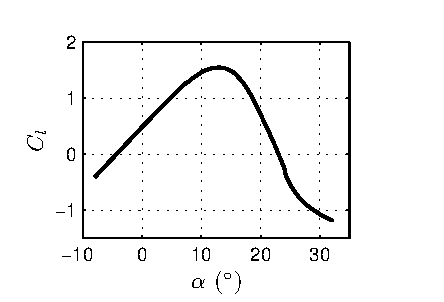
\includegraphics{NACA_4412_Cl.pdf}
	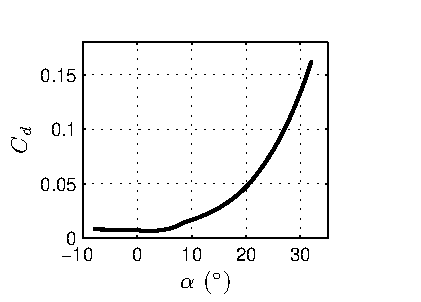
\includegraphics{NACA_4412_Cd.pdf}
	\caption{lift- een weerstandsco\"effici\"enten van een NACA 4412 profiel bij vari\"erende aanvalshoek}
	\label{fig:lift en weerstand ifv aanvalshoek}
\end{figure}
Bij kleine aanvalshoeken zien we dat de liftco\"effici\"ent ongeveer lineair stijgt met de aanvalshoek. tewijl de weerstandsco\"effici\"ent langzaam stijgt. Vanaf een gegeven aanvalshoek zal de liftkracht niet meer stijgen en op een gegeven moment terug beginnen dalen. Tegelijk stijgt de weerstandsco\"effici\"ent sterk. Dit gebeurt bij een hoek die veel kleiner is dan we zouden verwachten door middel van behoud van impuls.
\npar
Aan de bovenzijde van het profiel heerst een onderdruk die net na de aanvalsboord het grootst is. Aan de achterzijde van het profiel is de druk ongeveer de omgevingsdruk. Er is dus een stijgende druk aan de bovenzijde van het profiel. In combinatie met de gevormde grenslaag zorgt dit ervoor dat de stroming zal loshchten van het profiel. Er ontstaat een zog op omgevingsdruk dat ervoor zorgt dat de lift vermindert en de weerstand stijgt.
\npar
Uit de gelijkvormigheidstheorie weten we verder dat de krachten ook afhankelijk zullen zijn van het Reynolds getal: 
\begin{eqnarray}
	C_d &=& C_d(\text{Re}) \\
	C_l &=& C_l(\text{Re})
\end{eqnarray}
Deze effecten koemen echter pas tot uiting bij verandering van het Reynoldsgetal over meerdere grootte ordes en hoeven bij de meeste toepassingen niet in rekening worden gebracht.
